%PREÁMBULO
\documentclass[a4paper]{article}
\usepackage[spanish]{babel}
\usepackage[utf8]{inputenc}
\usepackage[pdftex]{graphicx}
\usepackage{hyperref} %Permite poner links
\parindent=0.5cm %Modificar el tamaño de la sangría
\parskip=0.5cm %Modificar el espaciado entre párrafos
\usepackage{float} %Movimiento de tablas y gráficos
\usepackage[lmargin=2.5cm,rmargin=2.5cm,top=2.5cm,bottom=2.5cm]{geometry} %Márgenes
\usepackage{natbib} %Paquete para que en el apartado de referencias no aparezcan los nombres por duplicado.
\usepackage{adjustbox}

%1.Encabezado
\usepackage{fancyhdr}
\pagestyle{fancy}
\fancyhead{} %Elimina el texto predeterminado del encabezado fancy
\fancyhead[C]{El camarón \textit{Palaemon serratus}} %Texto del encabezado
\renewcommand{\headrulewidth}{0.25pt} %Grosor de la línea

%2.Pie de página
\fancyfoot{} %Elimina el texto predeterminado del pie de página
\fancyfoot[R]{\thepage} %Comando para la numeración de página
\fancyfoot[L]{Jorge Garrido Bautista}

%COMIENZO DEL DOCUMENTO
\begin{document}

%Página inicial para el título del artículo y el autor
\begin{titlepage}
\begin{center}
\vspace*{5\baselineskip} %Espacio vertical
{\LARGE \textbf{Biología del camarón \textit{Palaemon serratus}\\(Pennant, 1777)}}
\vspace*{5\baselineskip}
\vfill %Este comando rellena con huecos vacíos el espacio entre la imagen y el último texto
{\large JORGE GARRIDO BAUTISTA}\\[1cm]
Curso de LaTeX y Git. Darwin Eventur\\
\textit{Texto adaptado a partir de mi TFM}
\end{center}
\end{titlepage}

%Segunda página inicial para el abstracts
\begin{titlepage}
\begin{abstract}
Repositorio:\\
\url{https://github.com/JorgeGarridoBautista/Proyecto_Final}\\
\\El camarón \textit{Palaemon serratus} (Pennant, 1777) es un crustáceo decápodo de la familia Palaemonidae que se distribuye por las costas del este del océano Atlántico y mar Mediterráneo. Su rápido desarrollo y su larga secuencia de estadios larvarios son características de interés para el estudio de los genes que intervienen, de forma directa o indirecta, en los procesos de muda o ecdisis y en la determinación o diferenciación sexual. En el presente artículo se hablará brevemente de todos estos aspectos.\\
\\Palabras clave: muda, ecdisis, biología básica, camarón, \textit{Palaemon serratus}
\end{abstract}
\end{titlepage}

%Comienzo del CUERPO DEL ARTÍCULO
\begin{titlepage}
\tableofcontents
\end{titlepage}

\section{Biología básica de \textit{Palaemon serratus}}
\subsection{Morfología y reproducción}
El camarón \textit{Palaemon serratus} (Pennant, 1777) es un crustáceo decápodo de la familia Palaemonidae que se caracteriza por su color casi transparente interrumpido por un pereion de líneas longitudinales rojizas que empiezan en el rostro y terminan en el borde posterior. Además de esto, también se distingue de otras especies coetáneas por la presencia de anillas amarillas y rojas en las patas \citep{Zariquiey1968}. Sin embargo, se ha observado que estas líneas rojas abdominales pueden estar ausentes en individuos que habitan aguas turbias \citep{Gonzalez2006}. El nombre de \textit{Palaemon serratus} deriva de su rostrum serrado: se bifurca en su punta y posee un número determinado de dientes en su parte dorsal y ventral \citep{Gonzalez2006}. \textit{P. serratus} se distribuye por el océano Atlántico Oriental, desde Cabo Blanco en la costa de Mauritania hasta Dinamarca en el norte de Europa; el Atlántico central (islas Azores) y el mar Mediterráneo, desde el estrecho de Gibraltar hasta las costas de Egipto e Israel \citep{Zariquiey1968, Felicio2002}.\par Es una especie bentónica que habita las zonas intermareales ---llegando hasta los 50 metros de profundidad--- de fondos rocosos o arenosos cubiertos de macroalgas y fanerógamas marinas \citep{Felicio2002}. Es una especie omnívora \citep{Forster1951} y presenta cierto dimorfismo sexual, ya que las hembras son más grandes y pesadas que los machos \citep{Guerao1995}. Es una especie que posee fecundación interna y un ciclo de vida corto: la media de edad de \textit{P.serratus} son 3 años \citep{Felicio2002}. La época reproductora es entre enero y mayo, aunque en las costas del sur de España se alarga de noviembre a agosto debido a una mayor temperatura \citep{Rodriguez1981, Figueras1986, Felicio2002}. En época reproductora los adultos migran desde aguas continentales a áreas costeras para emparejarse y reproducirse \citep{Gonzalez2014}.

\subsection{Desarrollo larvario}
El desarrollo larvario de \textit{P. serratus} ha sido estudiado por varios autores con el fin de identificar sus diferentes estadios larvarios. Los estadios larvarios de esta especie, y en general de los carídeos, se denominan zoeas. Las zoeas se caracterizan por el uso de apéndices torácicos para nadar llamados exópodos. Hasta la fecha no se han establecido los estadios de zoea de \textit{P. serrstus} \citep{Gonzalez2001}, pero muchos autores coinciden en que \textit{P. serratus} posee entre siete y nueve estadios larvarios planctónicos diferentes (tabla 1) \citep{Fincham1986, Ramonell1987}. Tanto la temperatura como la salinidad juegan un papel importante en el desarrollo de las zoeas ya que afectan a su tasa metabólica y crecimiento \citep{Gonzalez2014}. La muda de las zoeas ocurre en la columna de agua de las zonas litorales \citep{Forster1951} y la larga secuencia de estadios larvarios permite una dispersión amplia y eficaz de \textit{P. serratus} \citep{Fincham1986}.\par Los individuos que alcanzan el último estadio de zoea sufren metamorfosis a los 20-30 días para convertirse en decapoditos \citep{Bellon1978}. El estadio de decapodito es el último estadio larvario que precede al primer estadio juvenil \citep{Anger2001} y se caracteriza por la transición de la función natatoria de los pereiópodos en zoeas a los pleópodos en decapoditos. El decapodito es por tanto una forma transitoria del modo de vida planctónico al bentónico. Tras el estadio de decapodito, el organismo entra en una fase transitoria donde los caracteres larvarios desaparecen gradualmente y los caracteres juveniles comienzan a aparecer tras varias mudas \citep{Anger2001}. Durante el desarrollo larvario y el crecimiento de juveniles y adultos se producen varios cambios morfológicos y fisiológicos. En zoeas el crecimiento da lugar a la aparición de segmentos posteriores al caparazón con ocho pares de apéndices natatorios; en juveniles las branquias adquieren función osmorreguladora; y el tracto digestivo y aparato mandibular sufren cambios morfológicos \citep{Factor1981, Bouaricha1994, Ruppert1996}.

\begin{adjustbox}{max width=\textwidth}
\begin{tabular}{|l|c|c|}
\hline 
Especie & Estadios larvarios & Referencia\\
\hline
\textit{Leander (Palaemon) serratus} & Z1-Z9 & Sollaud (1912)\\
\hline
\textit{Leander (Palaemon) serratus} & Z1-Z9 & Sollaud (1923)\\
\hline
\textit{Palaemon serratus} & Z1-Z8 & Carli (1978)\\
\hline
\textit{Palaemon serratus} & Z1-Z9 & Fincham (1983)\\
\hline
\textit{Palaemon serratus} & Z1-Z9 & Fincham y Figueras (1986)\\
\hline
\textit{Palaemon serratus} & Z1-Z6 & Yagi (1986)\\
\hline
\textit{Palaemon serratus} & Z1-Z7 & Ramonell (1987)\\
\hline
\textit{Palaemon serratus} & Z1-Z8 & Barnich (1996)\\
\hline
\end{tabular}
\end{adjustbox}

\textbf{Tabla 1.} Estadios de zoea de \textit{Palaemon serratus} según varios autores. Nota: los distintos estadios de zoea se represetan como Z. Adaptado a partir de \citep{Gonzalez2001}.\par

\section{La muda o ecdisis de \textit{Palaemon serratus}}
El proceso de ecdisis provoca cambios metabólicos, citológicos y etológicos: incremento en el consumo de oxígeno, acumulación de lipoproteínas y gránulos acidófilos en las células epidérmicas o consumo del viejo exoesqueleto tras la ecdisis \citep{Reeve1969}. El proceso completo de muda o ecdisis se divide en cuatro fases en función del estado del tegumento: proecdisis, ecdisis, postecdisis e intermuda (figura \ref{Figura 1}). Durante la proecdisis se acumulan reservas alimenticias y aumenta la concentración de calcio en la hemolinfa debido a la reabsorción de éste de la procutícula \citep{Arlot1986}. El calcio reabsorbido se acumula en estructuras denominadas gastrolitos que serán disueltos en la postecdisis y usados como fuente mineral para la nueva cutícula \citep{Tom2014}. Durante la proecdisis también se produce el fenómeno de apólisis: separación de la epidermis de la vieja cutícula gracias a la acción de enzimas proteolíticas y quitinolíticas \citep{Spindler1990}. Durante esta fase se sintetizan además las nuevas epicutícula y exocutícula por parte de las células epidérmicas \citep{Tom2014}. La ecdisis \textit{per se} es un proceso breve caracterizado la ingesta de agua y la salida del organismo del viejo exoesqueleto o exuvia. Durante la postecdisis se sintetiza la nueva endocutícula y se produce la calcificación de la procutícula, además de perder el agua ingerida anteriormente. El organismo también encoge de tamaño para permitir el crecimiento durante la posterior intermuda \citep{Hickman2002}. Por último, en el período de intermuda el organismo crece y la endocutícula aumenta de grosor, se endurece y se calcifica progresivamente.

\begin{figure}[t]
\begin{center}
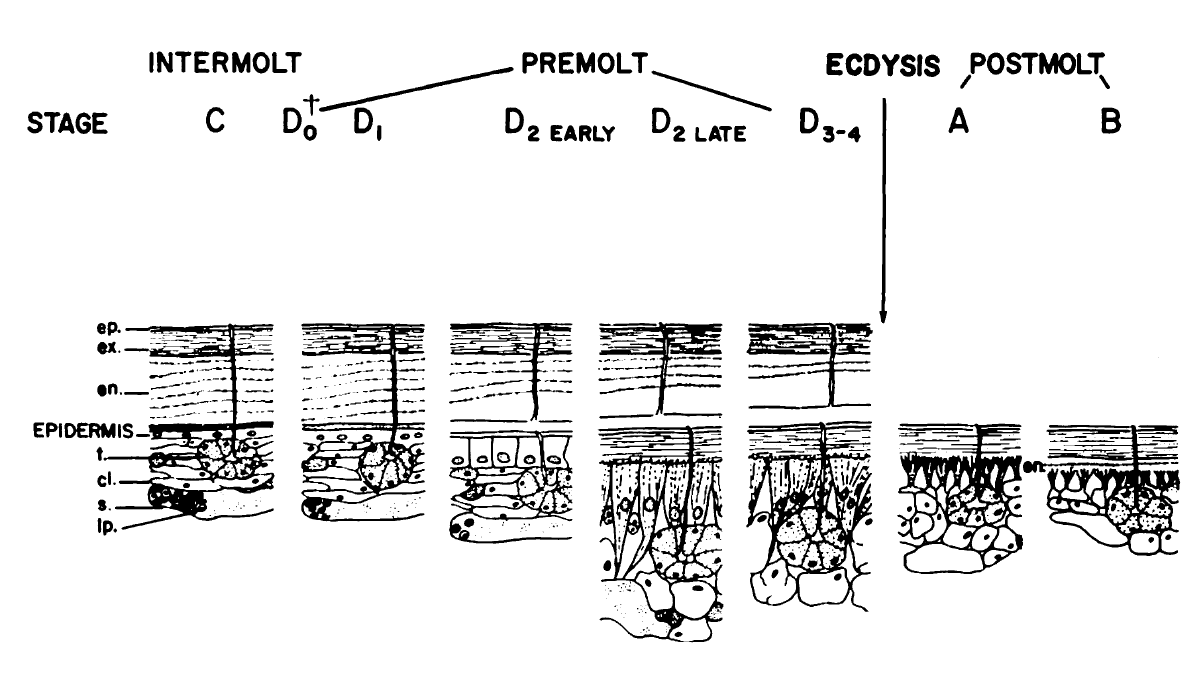
\includegraphics[width=1\textwidth]{Imagen 1 (Skinner1962).png} 
\caption{Fases del proceso de muda. La fase de proecdisis se subdivide a su vez en cuatro etapas: D{\footnotesize 0}, donde ocurre la apólisis y se regeneran las extremidades autotomizadas si las hubiera; D{\footnotesize 1}, donde se produce la reabsorción de calcio de la procutícula; D{\footnotesize 2}, donde ocurre la síntesis de la epicutícula y exocutícula y aumenta el consumo de oxígeno; D{\footnotesize 3} y D{\footnotesize 4}, sin síntesis de cutícula y caracterizadas por el cambio de color de la hemolinfa. La fase de postecdisis se subdivide en dos etapas: en la B se produce la síntesis de la endocutícula, que continuará durante la fase de intermuda. Abreviaciones: ep, epicutícula; ex, exocutícula; en, endocutícula; t, glándula; cl, célula de Leydig; s, capilar; lp, lipoproteínas. Figura extraída de Skinner, 1962.}
\label{Figura 1}
\end{center}
\end{figure}

\subsection{Regulación hormonal de la muda}
Todo el proceso de muda está bajo control endocrino \citep{Techa2013}. Se ha comprobado que este mecanismo de control hormonal es similar tanto en zoeas como en los estadios juveniles y adultos, y que este control a su vez está asociado al desarrollo de sus glándulas y órganos asociados \citep{Webster1991}. Aunque el conocimiento de la regulación hormonal de la muda está todavía incompleto, sí que se conoce bastante bien el papel antagónico que juegan dos hormonas esenciales.\par Por un lado se encuentra la hormona inhibidora de la muda, que es secretada y almacenada posteriormente en la glándula sinusal \citep{Hartnoll2001}. Esta hormona provoca la reducción de los niveles de síntesis de su antagónico, los ecdisteroides \citep{Anger2001, Hartnoll2001}. Los ecdisteroides son hormonas esteroideas que inducen el proceso de muda y están presentes, principalmente, en dos formas: ecdisona y 20-hidroxiecdisona (ésta última es la forma fisiológicamente activa) \citep{Das2016}. La interacción entre ambas hormonas crea los ciclos de muda: la ecdisteroidogénesis se inhibe durante la fase de intermuda debido a la acción constante de la hormona inhibidora de la muda, se activa en proecdisis y se vuelve a reprimir en postecdisis \citep{Zou2004}. En la interacción entre estas dos hormonas intervienen otras. Algunos ejemplos son la hormona hiperglucémica de crustáceos, que moviliza la glucosa a los tejidos durante respuestas a estrés \citep{Hartnoll2001} e inhibe la síntesis de ecdisteroides; el metil farnesoato, una hormona sesquiterpenoide de estructura similar a la hormona juvenil de insectos que estimula la vitelogénesis en la etapa adulta \citep{Hartnoll2001} y estimula la producción de ecdisteroides. Otra hormona implicada indirectamente en la ecdisteroidogénesis es la hormona inhibidora del órgano mandibular, un neuropéptido que reprime una de las enzimas implicadas en la biosíntesis del metil farnesoato \citep{Wainwright1996}. Una última hormona a destacar por su importancia en la calcificación de la cutícula es la calcitonina. Se ha visto que la calcitonina hemolinfática alcanza su máximo en postecdisis, cuando la concentración de calcio en hemolinfa es mínima y ocurre la calcificación; mientras que el mínimo de calcitonina ocurre durante la intermuda y la proecdisis temprana, cuando la concentración de calcio es máxima \citep{Arlot1986}.

\subsection{Regulación genética de la muda}
La regulación genética de la muda es aun más complicada que la hormonal y permanece en constante investigación. La 20-hidroxiecdisona es el regulador central en la formación de la cutícula ya que inicia la cascada de activación génica que provoca la ecdisis. En un inicio la 20-hidroxiecdisona se une a sus dos receptores nucleares y cuando se forma el complejo, éste se une a elementos de respuesta a ecdisona y a promotores de genes de respuesta a ecdisteroides, que codifican para factores transcripcionales \citep{Puthumana2017}. Estos factores transcripcionales se clasifican como genes tempranos y regulan la activación de genes involucrados en el proceso de ecdisis, los cuales se conocen como genes tardíos. Algunos de los factores transcripcionales tempranos inducidos por la 20-hidroxiecdisona son E74, E75 o el factor 11 asociado al complejo SAGA \citep{Qian2014}. SGF11 es requerido para la expresión de algunos genes de respuesta a ecdisona como EcR o E74, mientras que E74 y E75 provocan la expresión o represión de genes tardíos implicados en la proliferación celular, diferenciación de tejidos y muda \citep{Dubro2005}. Algunos de los genes tardíos reprimidos por E75 durante la proecdisis son la catepsina-L, una proteasa involucrada en la degradación de proteínas durante la ecdisis, o la hemocianina, una proteína hemolinfática que transporta el oxígeno requerido por el proceso de muda \citep{Qian2014}. La 20-hidroxiecdisona también induce, a través de E75, la transcripción de genes tardíos que codifican para quitinasas y Acetilglucosaminidasas, enzimas implicadas en la degradación o hidrólisis de la quitina durante la apólisis \citep{Zou2004}). Por otro lado, durante la proecdisis se induce la expresión de quitina-sintetasas que sintetizan la quitina de la nueva cutícula una vez se ha producido la apólisis \citep{Qian2014}. Durante la postecdisis se ha visto que se induce también la expresión de actina F, tubulina, troponina y esquelemina (proteínas del citoesqueleto o asociadas a éste). Sus cambios de expresión podrían estar relacionados con el incremento de los niveles de ecdisteroides y con el aumento de tamaño del organismo durante la ecdisis cuando se produce la ingesta de agua \citep{Tom2014}.\par Fórmula matemática de crecimiento exponencial (por meter alguna):\par 

\begin{displaymath}
\frac{dN}{dT}=r*N
\end{displaymath}

\section{Bibliografía}
\bibliography{Biblio}
\bibliographystyle{apalike} %Bibliografía estilo APA. Cuando se introducen las referencias bibliográficas (.bib) hay que actualizar varias veces para que salga el formato correcto y todas las citas. Se hace presionando F6 y F11 varias veces seguidas.

\end{document}
